\section{Undersøkelser}
\label{sec:concept}


\subsection{Realisering av krets}
\label{subsec:realisering_av_krets}

Først realiseres kretsen, for enkelhetens skyld deles systemet inn i 3 delsystemer som vist i figur \ref{fig:blockdiagram}

\begin{figure}[!hbt]
	\centering
	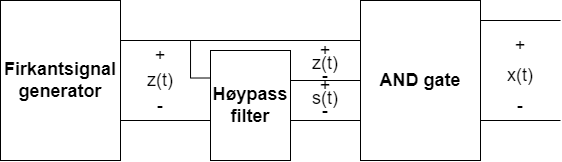
\includegraphics[scale=0.5]{./Images/02Concept/01blokkdiagram.png}
	\caption{Blokkdiagram av kretsen.}
    \label{fig:blockdiagram}
\end{figure}

Det chippen CD4011UBE blir brukt i dette prosjektet, da den har 4 NAND gates så blir firkantsignalgenerator fra figur \ref{fig:blockdiagram} realisert med 2 NAND gater, motstand og kondensator som vist i figur \ref{fig:firkantsignalgenerator}.

\begin{figure}[!hbt]
	\centering
	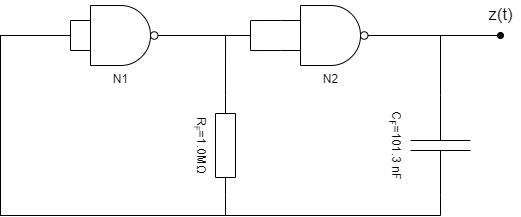
\includegraphics[scale=0.5]{./Images/02Concept/02firkantsignal.png}
	\caption{Kretsdiagram av firkantsignalgenerator.}
    \label{fig:firkantsignalgenerator}
\end{figure}

Grunnen til at dette funker er at NAND vil virke som en inverter når begge inngangene er det samme. Virkemåten til kretsen blir beskrevet i notatet \cite{instituttforelektroniskesystemntnu_2022_ertykt}. Det blir også berskrevet at perioden til klokkegeneratoren er gitt
ved:

\begin{equation}
	T=2ln(3)\tau _F
	\label{eq:T}
\end{equation}

Der $\tau _F$ er gitt ved:

\begin{equation}
	\tau _F = R_F C_F 
	\label{eq:tau}
\end{equation}

Med kretsen fra figur \ref{fig:firkantsignalgenerator} ble signalet fra figur \ref{fig:firkantsignal}

\begin{figure}[!hbt]
	\centering
	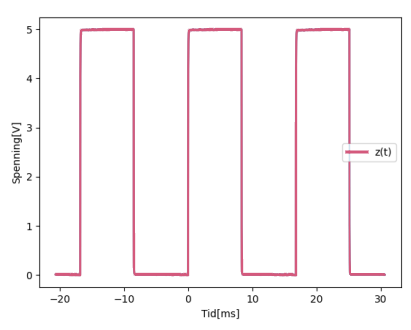
\includegraphics[scale=0.4]{./Images/02Concept/03plotfirkant.png}
	\caption{Firkantsignal $z(t)$.}
    \label{fig:firkantsignal}
\end{figure}

Videre blir firkantsignalet sendt inn i et høypassfilter som illustrert i figur \ref{fig:høypassfilter}.

\begin{figure}[!hbt]
	\centering
	\includegraphics[scale=0.5]{./Images/02Concept/04høypassfilter.png}
	\caption{Høypassfilteret.}
    \label{fig:høypassfilter}
\end{figure}

Med delsystemene fra figur \ref{fig:firkantsignalgenerator} og figur \ref{fig:høypassfilter} vis i figur \ref{fig:Impulsgenerator} ble signalet $x(t)$ målt og plottet i figur \ref{fig:Impulssignalet}

\begin{figure}[!hbt]
	\centering
	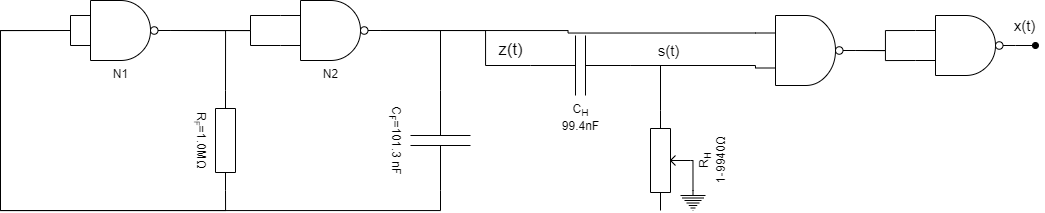
\includegraphics[scale=0.3]{./Images/02Concept/05begge.png}
	\caption{Impulsgenerator.}
    \label{fig:Impulsgenerator}
\end{figure}

\begin{figure}[!hbt]
	\centering
	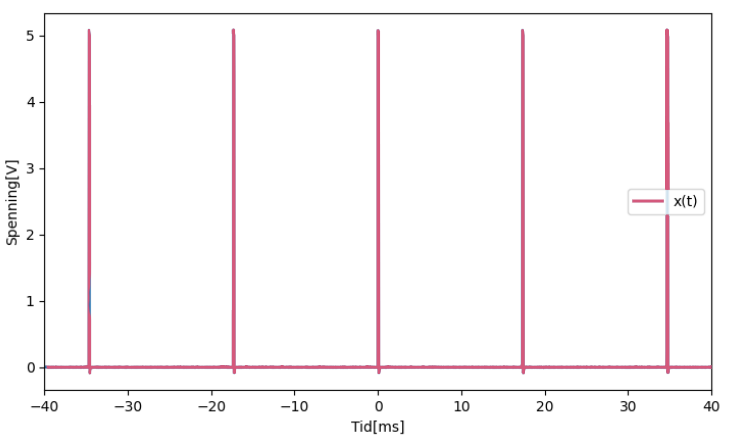
\includegraphics[scale=0.3]{./Images/02Concept/06plotimpuls.png}
	\caption{Impulssignalet $x(t)$.}
    \label{fig:Impulssignalet}
\end{figure}

\begin{figure}[!hbt]
	\centering
	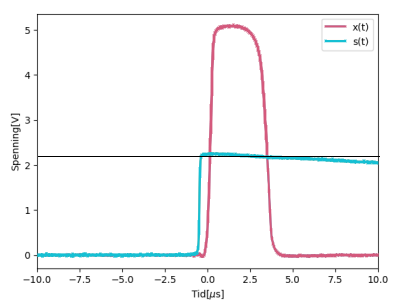
\includegraphics[scale=0.5]{./Images/02Concept/07beggeplotimpulsogmer.png}
	\caption{Forholdet mellom $s(t)$, $x(t)$ og terkskelspenningen til NAND gaten $V_t$.}
    \label{fig:Forholdet}
\end{figure}

Her ser man at systemet virker som forventet. $x(t)$  er en puls som avhenger av hvor mye av signalet $s(t)$ som er over terkskelspenningen $V_t$ til NAND-gaten som illustrert i figur \ref{fig:Forholdet}. Dermed har det blitt bevist at det er mulig å implementere ideen ved hjelp av en CMOS-krets av typen CD4011UBE med motsander og kondensatorer.

\subsection{Videre undersøkelse av impulssignalet}
\label{videre_undersøkelse}

For å videre teste hvor korte pulser som er praktisk mulig å få til med systemet i figur \ref{fig:Impulsgenerator} justeres motstanden $R_H$. Det ble observert at når $R_H < 340\Omega$ ble signalet ustabilt og lite målbart. Ved $R_H \approx 350\Omega$ ble pulsbredden målt til $3\mu s$ som vis i figur \ref{fig:kortpuls}

\begin{figure}[!hbt]
	\centering
	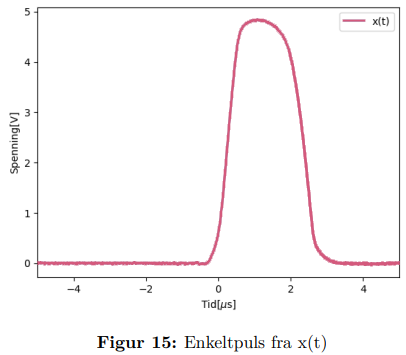
\includegraphics[scale=0.3]{./Images/02Concept/08puls.png}
	\caption{Korteste målte puls av $x(t)$.}
    \label{fig:kortpuls}
\end{figure}

Det observeres at firkantsignalet får mindre definerte skarpe kanter og blir mer avrundet ettersom pulsbredden minkes.

Fra presentasjonen \cite{lindem_2012_uke} får man at 

\begin{equation}
	v_c(t) = v(\infty)-(v(0)-v(\infty))e^{\frac{-t}{\tau_s}}
\end{equation}

der man videre kan skrive om til.

\begin{equation}
	t=-\tau _s \cdot ln \frac{v_{terskel}}{v_z}
\end{equation}

Her er $v_{terskel}$ terskelspenningen til NAND-gaten og $v_z$ er amplituden til firkantgeneratoren.

Ved å bruke de verdiene som er blitt brukt i kretsen så får vi en teoretisk pulsbredde på $2.8\mu s$. Dette ser ut til å stemme ganske greit overens med målte verdier.

\subsection{Videre undersøkelse av spekteret til impulssignalet}
\label{videre_undersøkelse_spekter}

Ved å måle spekteret til pulsene får man at frekvensinholdet er relativt flatt fra, til omtrent 0.5MHz der det gradvis krummer ned.

\begin{figure}[!hbt]
	\centering
	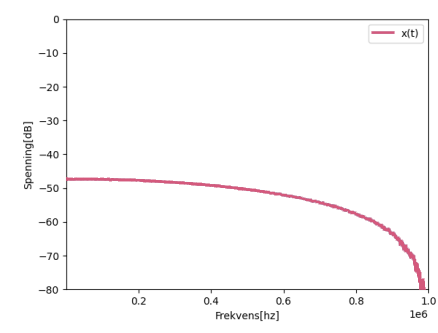
\includegraphics[scale=0.5]{./Images/02Concept/09spekter.png}
	\caption{Spektereret til $x(t)$.}
    \label{fig:spekter}
\end{figure}


\subsection{Test av Impulsgeneratoren på et RLC-båndpassfilter}
\label{test_impuls}

Med denne impulsgeneratoren skal vi prøve å finne impulsresponsen til et RLC-båndpassfilter med senterfrekvens $f_g = 350Hz$. Ved bruk av formelen for resonansfrekvens gitt ved

\begin{equation}
	f_0 = \frac{1}{2 \pi \sqrt{L_f C_f}}
\end{equation}

med utgangspunkt fra formelen for resonansfrekvens blir filteret realisert med $L_f = 0.210 H$ og $C_f=984nF$. 

\begin{figure}[!hbt]
	\centering
	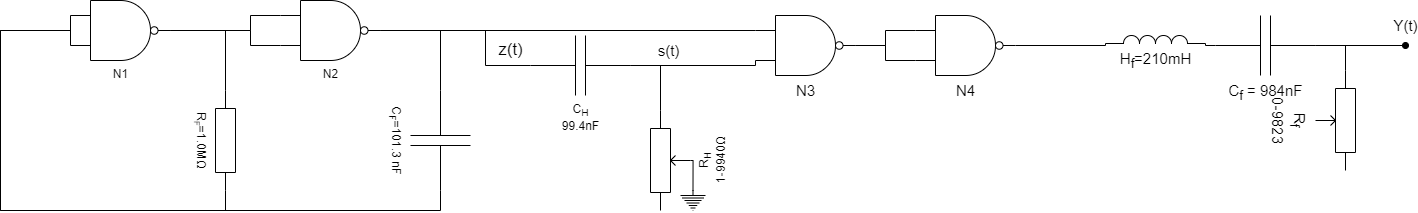
\includegraphics[scale=0.3]{./Images/02Concept/10alt.png}
	\caption{hele kretsen.}
    \label{fig:hele}
\end{figure}

Ved å sende impuls inn i et slikt RLC-filter vil både spolen og kondensatoren holde på energi og dytte den imellom seg da spolen vil motsette seg endring, mens kondensatoren lades opp og ut igjen. Denne energien vil gradvis redusseres som følge av motstands komponenten. vi vil dermed få et utgangssignal på formen av et sinc-finksjon som vis i figur \ref{fig:sinc}

\begin{figure}[!hbt]
	\centering
	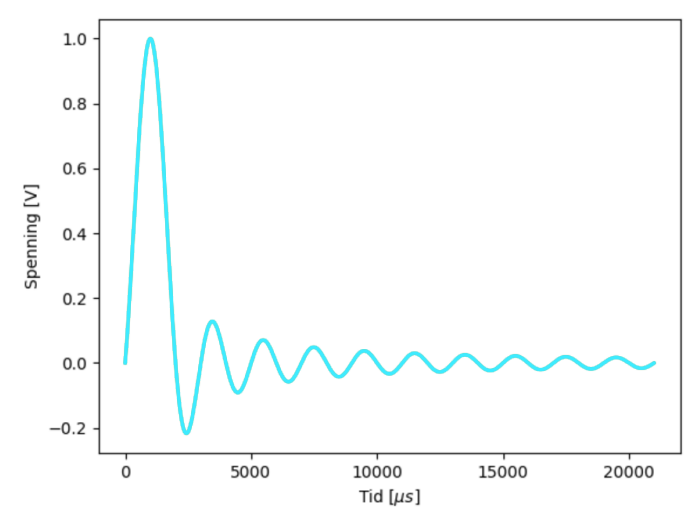
\includegraphics[scale=0.5]{./Images/02Concept/11sinc.png}
	\caption{Sinc-funksjon.}
    \label{fig:sinc}
\end{figure}

Videre har man at Q-faktoren er gitt ved

\begin{equation}
	Q=\frac{1}{R} \sqrt{\frac{L_f}{C_f}}
\end{equation}

\begin{figure}[!hbt]
	\centering
	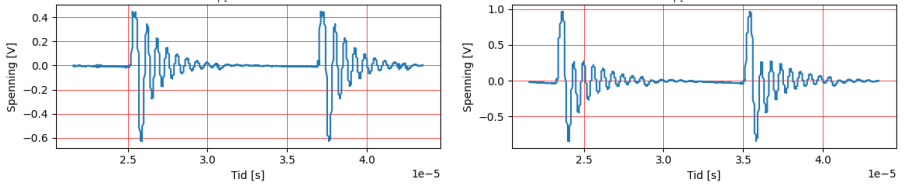
\includegraphics[scale=0.5]{./Images/02Concept/12sinccc.png}
	\caption{til venstre er det lav $R_f$ og høy $R_f$ til høyre.}
    \label{fig:sinccc}
\end{figure}

man kan se på impulsresponsen på figur \ref{fig:sinccc} at ved lav motstand gir høy Q-faktor som igjen fører til at signalet $y(t)$ bruker lenger tid på å dø ut, og motsatt for lav Q-faktor.

